\section{Hardware}\label{sec:hw}
\subsection{Diagrama en bloques general}
El sistema se compone de módulos funcionales que interactúan entre sí, estos son: el \emph{maestro}, el cual recibe los datos recibidos y los \emph{esclavos} que actualizan una matriz, en la figura \ref{fig:diagrama-bloques-general} se puede observar el diagrama en bloques de todo el sistema.

\begin{figure}[!ht]
	\centering
	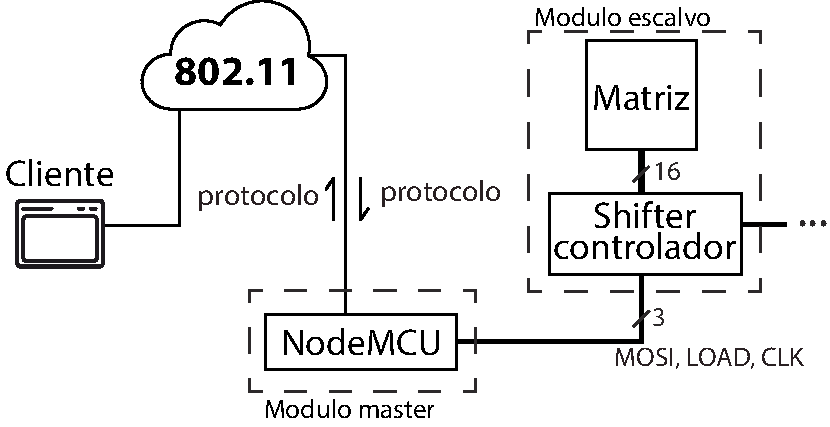
\includegraphics[width=\linewidth]{imagenes/hw/diagrama-bloques-general.pdf}
	\caption{Esquema general entre todos los componentes del sistema.}
	\label{fig:diagrama-bloques-general}
\end{figure}

\subsection{Fuente de alimentación}
El cartel requiere una alimentación de 5V de corrriente continua. Para esto se expone un conector hembra (de 5.5mm x 2.1mm), el cual se conecta a un transformador externo de 220V AC a 5V DC. El sistema no posee batería de ningún tipo.
%TODO: falta poner consumo

\subsection{Módulo maestro}
Como se mencionó anteriormente, este modulo se encarga de procesar los datos enviados desde el cliente y controlar los demás módulos.

Su componente principal es el microcontrolador NodeMCU, que integra un AI-Thinker ESP-12E (figura \ref{fig:foto-esp12e}), el cual contiene un SoC (\emph{System on Chip}) ESP8266EX (figura \ref{fig:esp8266ex}) de la empresa Espressif. El módulo NodeMCU es hardware libre, sin embargo, el ESP12E y el ESP8266EX no lo son.\cite{NodeMCU}

\begin{figure}[ht!]
	\begin{center}
		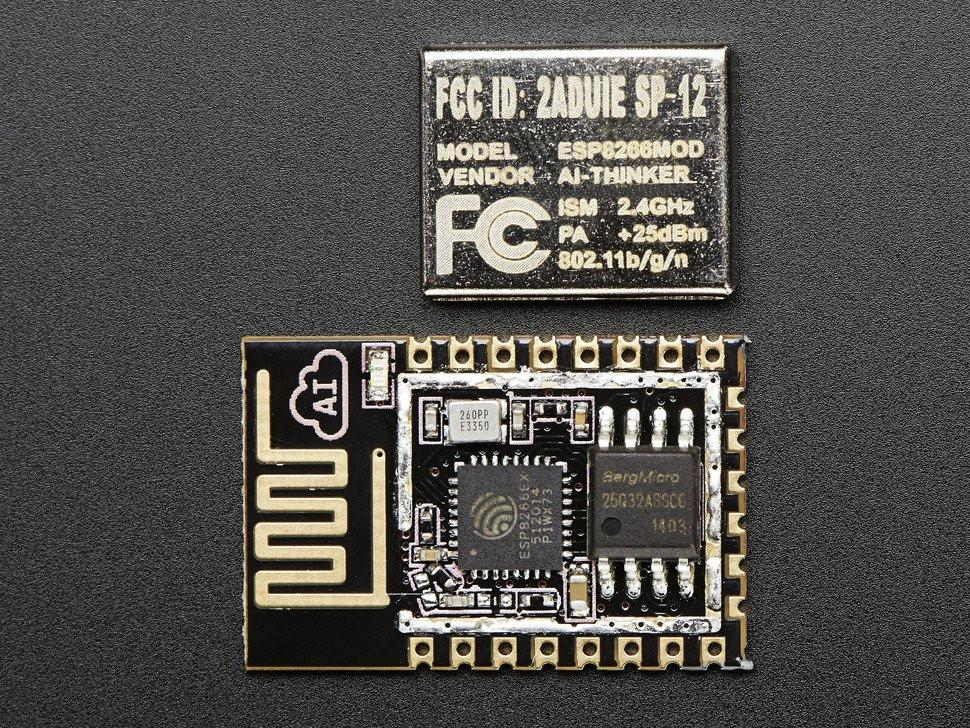
\includegraphics[width=8cm]{imagenes/esp12e-foto.jpg}
		\caption{Foto del módulo ESP12E sin su cubrimiento.}
		\label{fig:foto-esp12e}
	\end{center}
\end{figure}

\begin{figure}[ht!]
	\begin{center}
		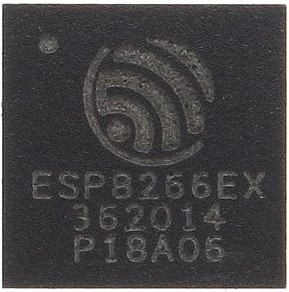
\includegraphics[width=3cm]{imagenes/esp8266ex.jpg}
		\caption{Foto del integrado ESP8266EX.}
		\label{fig:esp8266ex}
	\end{center}
\end{figure}

\begin{figure}[ht!]
	\begin{center}
		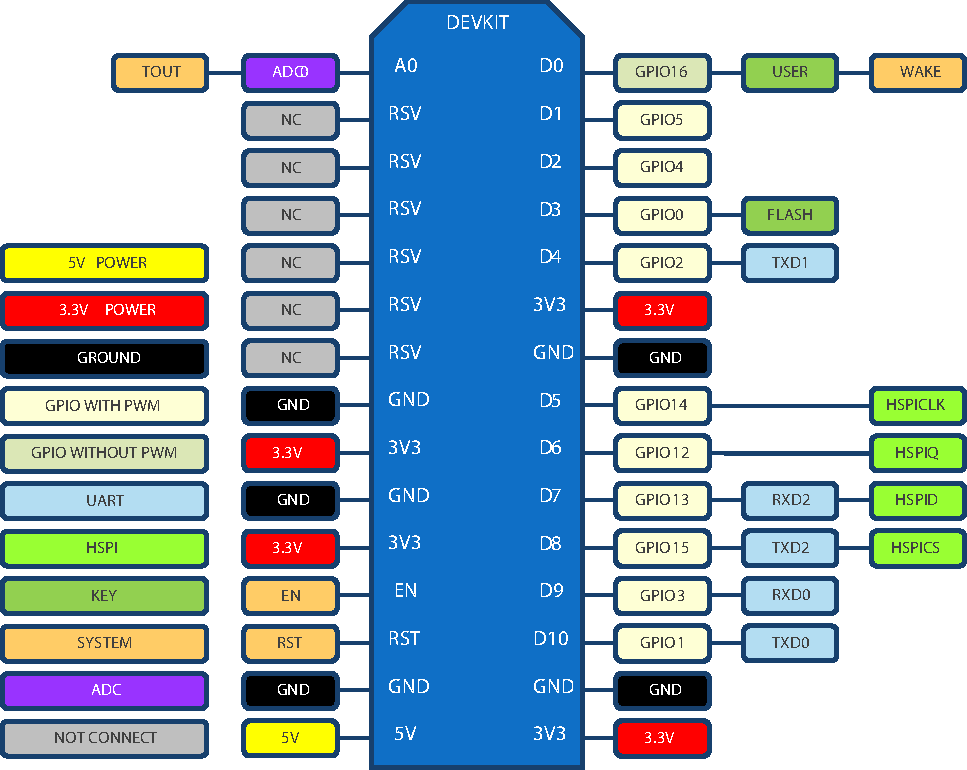
\includegraphics[width=0.95\textwidth]{imagenes/nodemcu-pinout.pdf}
		\caption{Asignación de pines del NodeMCU.}
		\label{fig:nodemcu-pinout}
	\end{center}
\end{figure}

Es importante tener en cuenta que el sistema no integra en su hardware directamente ni el ESP12E ni el ESP8266EX, sino que integra el NodeMCU, cuya asignación de pines se puede ver en la figura \ref{fig:nodemcu-pinout}.

El chip ESP8266EX combina un microcontrolador Tensillica Xtensa L106, un RISC de 32 bits corriendo a 80 Mhz, con funcionalidad WiFi. \cite{ESP8266Datasheet} El chip tiene memoria ROM con firmware no removible, y puede correr programas almacenados en flash externa. Para poder usar todas sus funcionalidades, se debe programar sobre firmware privativo desarrollado por Espressif, esto implica que el programa de usuario corre en simultáneo con el firmware (utilizando funciones disponibilizadas por el firmware) y el uso de la memoria de trabajo está sujeto a la versión del firmware. Según el datasheet del ESP8266EX, el usuario puede esperar tener disponible 50 KiB de RAM para alocar variables globales o utilizando la heap.
k

Como se mencionó anteriormente, se necesita de flash externa para correr programas. El módulo ESP-12S se encarga de proveer al ESP8266EX 4 MiB de memoria flash.

\subsection{Módulo esclavo}
Un modulo esclavo posee un driver MAX7219, que es el componente principal junto con una interfaz que permite conectarse a otro módulo esclavo o en su defecto al master.

\subsubsection{MAX7219}
El MAX7219 es un controlador compacto, de entrada y salida en serie de cátodo común que conectan, indirectamente, microcontroladores a LEDs numéricos de siete segmentos de hasta ocho dígitos, pantallas de gráfico de barras o, en este caso, 64 LED individuales dispuestos de forma matricial. Se incluye en el chip, un decodificador BCD, circuitos de multiplexación, controladores de segmentos y dígitos, y una RAM estática de 8x8 que almacena cada número, o en este caso, mapas de bits. Solo se necesita una resistencia externa para configurar la corriente para todos los LEDs.

Las matrices individuales se pueden actualizar sin reescribir toda la pantalla.

Su alimentación V\texttt{+} debe estar entre 4 y 5.5 Volts para su correcto funcionamiento. En cambio los voltaje de las entradas lógicas tienen una restricción de que un valor alto como mínimo debe ser 3.5V y un valor bajo debe ser como máximo 0.8V.

Las características principales que posee el chip integrado se enumeran a continuación:
\begin{itemize}
	\item Interfaz serie de 10 MHz.
	\item Control de segmento LED individual.
	\item Selección de dígitos Decode / No-Decode.
	\item Apagado de baja potencia de 150 microA (datos retenidos).
	\item Control de brillo digital y analógico.
	\item Pantalla borrada al encenderse.
	\item Unidad de visualización LED de cátodo común.
	\item SPI, QSPI, interfaz serie Microwire paquetes DIP y SO de 24 pines.
\end{itemize}

La disposición de los pines del MAX7219 se puede observar en la figura \ref{fig:MAX-pines} y la descripción de cada uno en la tabla \ref{table:MAX-pines}.

Es necesario prestar atención en el conexionado con respecto a los pines de tierra (GND) ya que ambos deben estar conectados para el driver pueda funcionar correctamente, ambas estan al lado izquierdo de la figura \ref{fig:MAX-pines} (Pin 4 y 9).

Por otro lado, el MAX7219 tiene un pin denominado DOUT (pin 24) se utiliza para encadenar varios MAX7219 y de esta forma pasar la información al que esta directamente conectado, éste pin nunca tiene alta impedancia.

\begin{figure}[htp!]
	\centering
	\begin{center}
	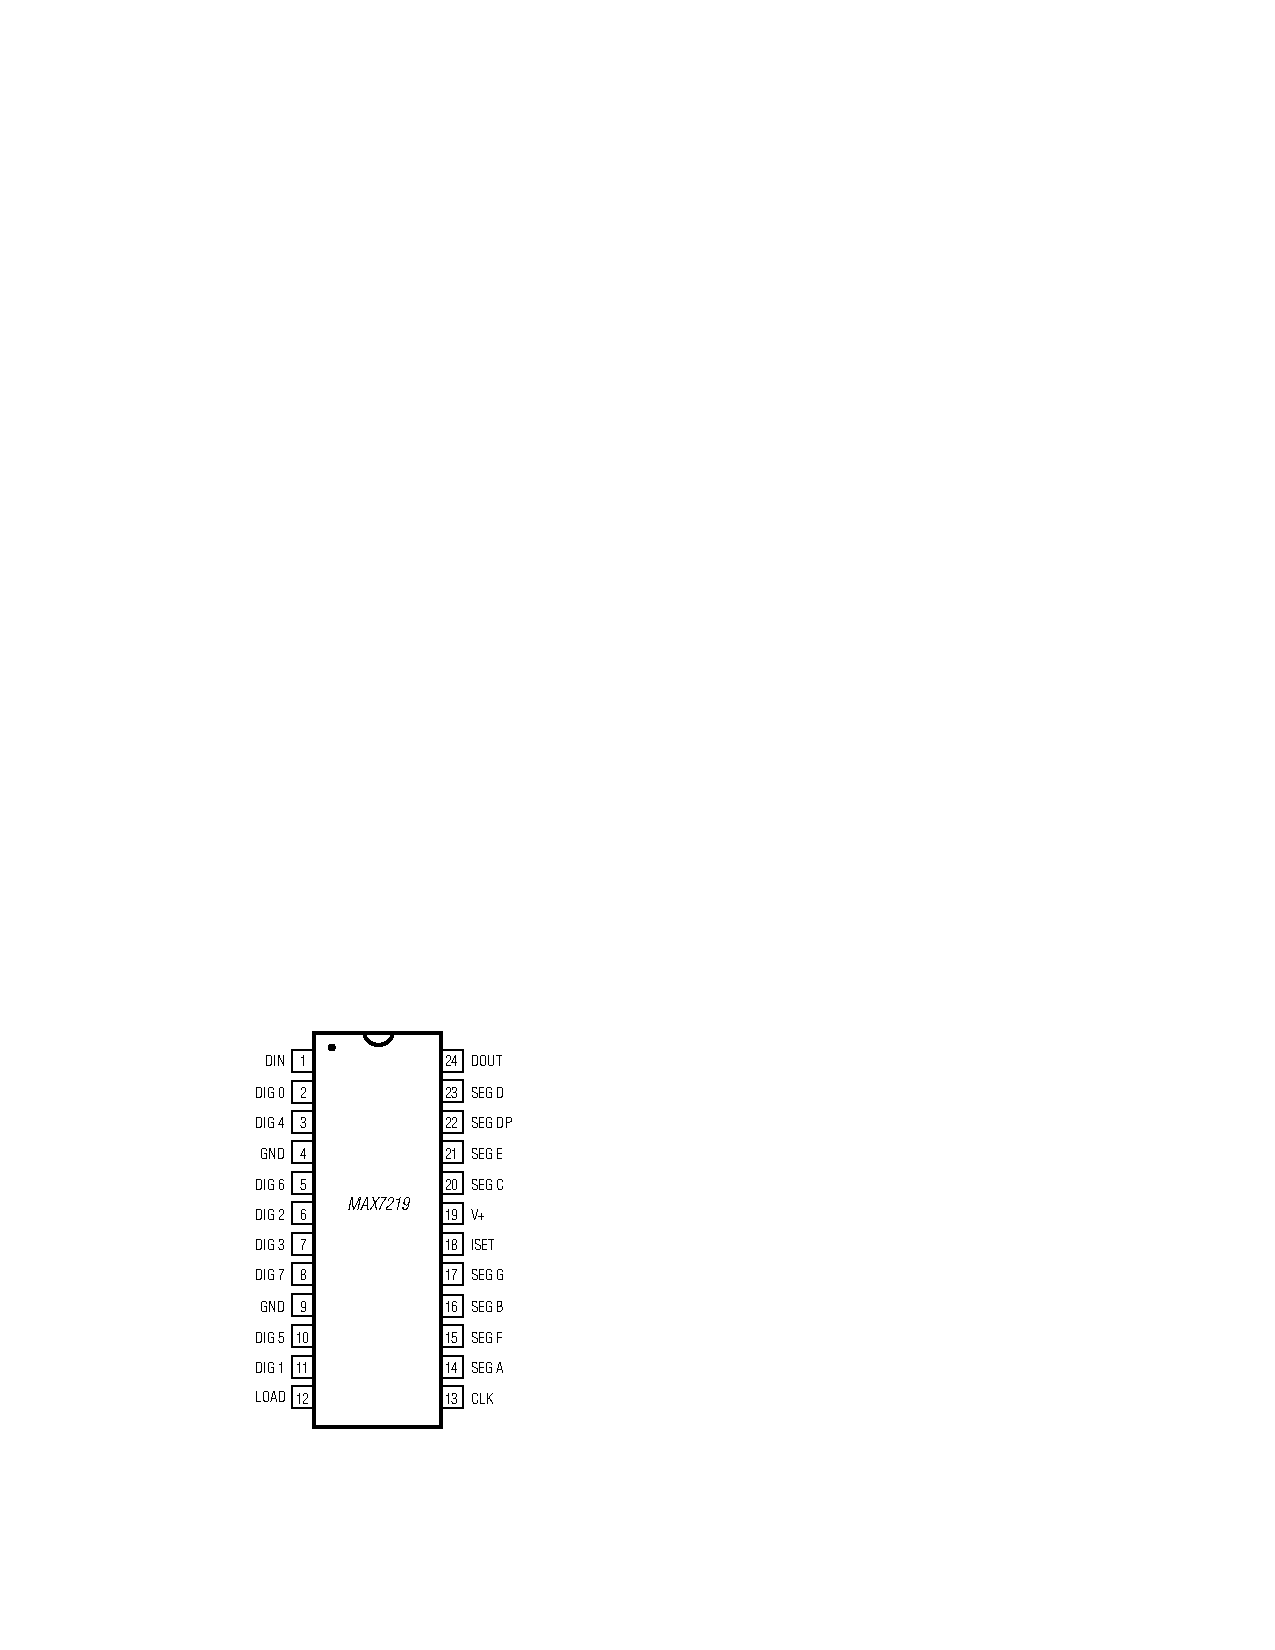
\includegraphics[scale=1.2]{imagenes/hw/max.pdf}
	 \caption{Configuración de pines del chip MAX7219.}
	  \label{fig:MAX-pines}
	\end{center}
\end{figure}

\begin{table}[htp!]
\centering
\caption{Descripción de los pines del MAX7219}
\label{table:MAX-pines}
\begin{tabular}{C{10mm} C{14mm} L{108mm}}
\hline
Pin               & Nombre          & Función    \\ \hline
1                 & DIN             & Pin de datos seriales. Los datos son cargados en el registro de 16 bits en cada flanco ascendente del clock. \\
2, 3, 5–8, 10, 11 & DIG 0 - DIG 7    & Líneas de transmisión de ocho dígitos que absorben corriente del cátodo común de la pantalla. El MAX7219 deja en V+ cuando esta apagado. Los dígitos están en alta impedancia cunado se apaga.\\
4, 9              & GND             & Tierra.\\
12                & LOAD            & Pin de control. Los últimos 16 bits del Serial Data son cargados en el flanco ascendente. \\
13                & CLK             & Pin de clock serial. En cada flanco ascendente, los datos sin shifteados dentro de un registro interno. En cada flanco descendente los datos salen de DOUT. En el MAX7221, la entrada CLK está activa solo mientras LOAD está baja. \\
14–17, 20-23      & SEG A–SEG G, DP & Las unidades de siete segmentos y el punto decimal impulsan la fuente de corriente a la pantalla. Cuando un controlador de segmento está apagado, se conecta a GND.\\
18                & ISET            & Conectar a  $V_{DD}$ a través de una resistencia ($R_{SET}$) para configurar la corriente que pueda entregar a los dígitos y segmentos. \\
19                & V+              & Fuente positiva de corriente, conectar a 5 V. \\
24                & DOUT            & Salida de datos en serie. Los datos en DIN son válidos en DOUT 16.5 ciclos de reloj más tarde. \\ \hline
\end{tabular}
\end{table}

\begin{figure}[htp!]
\centering
\begin{center}
	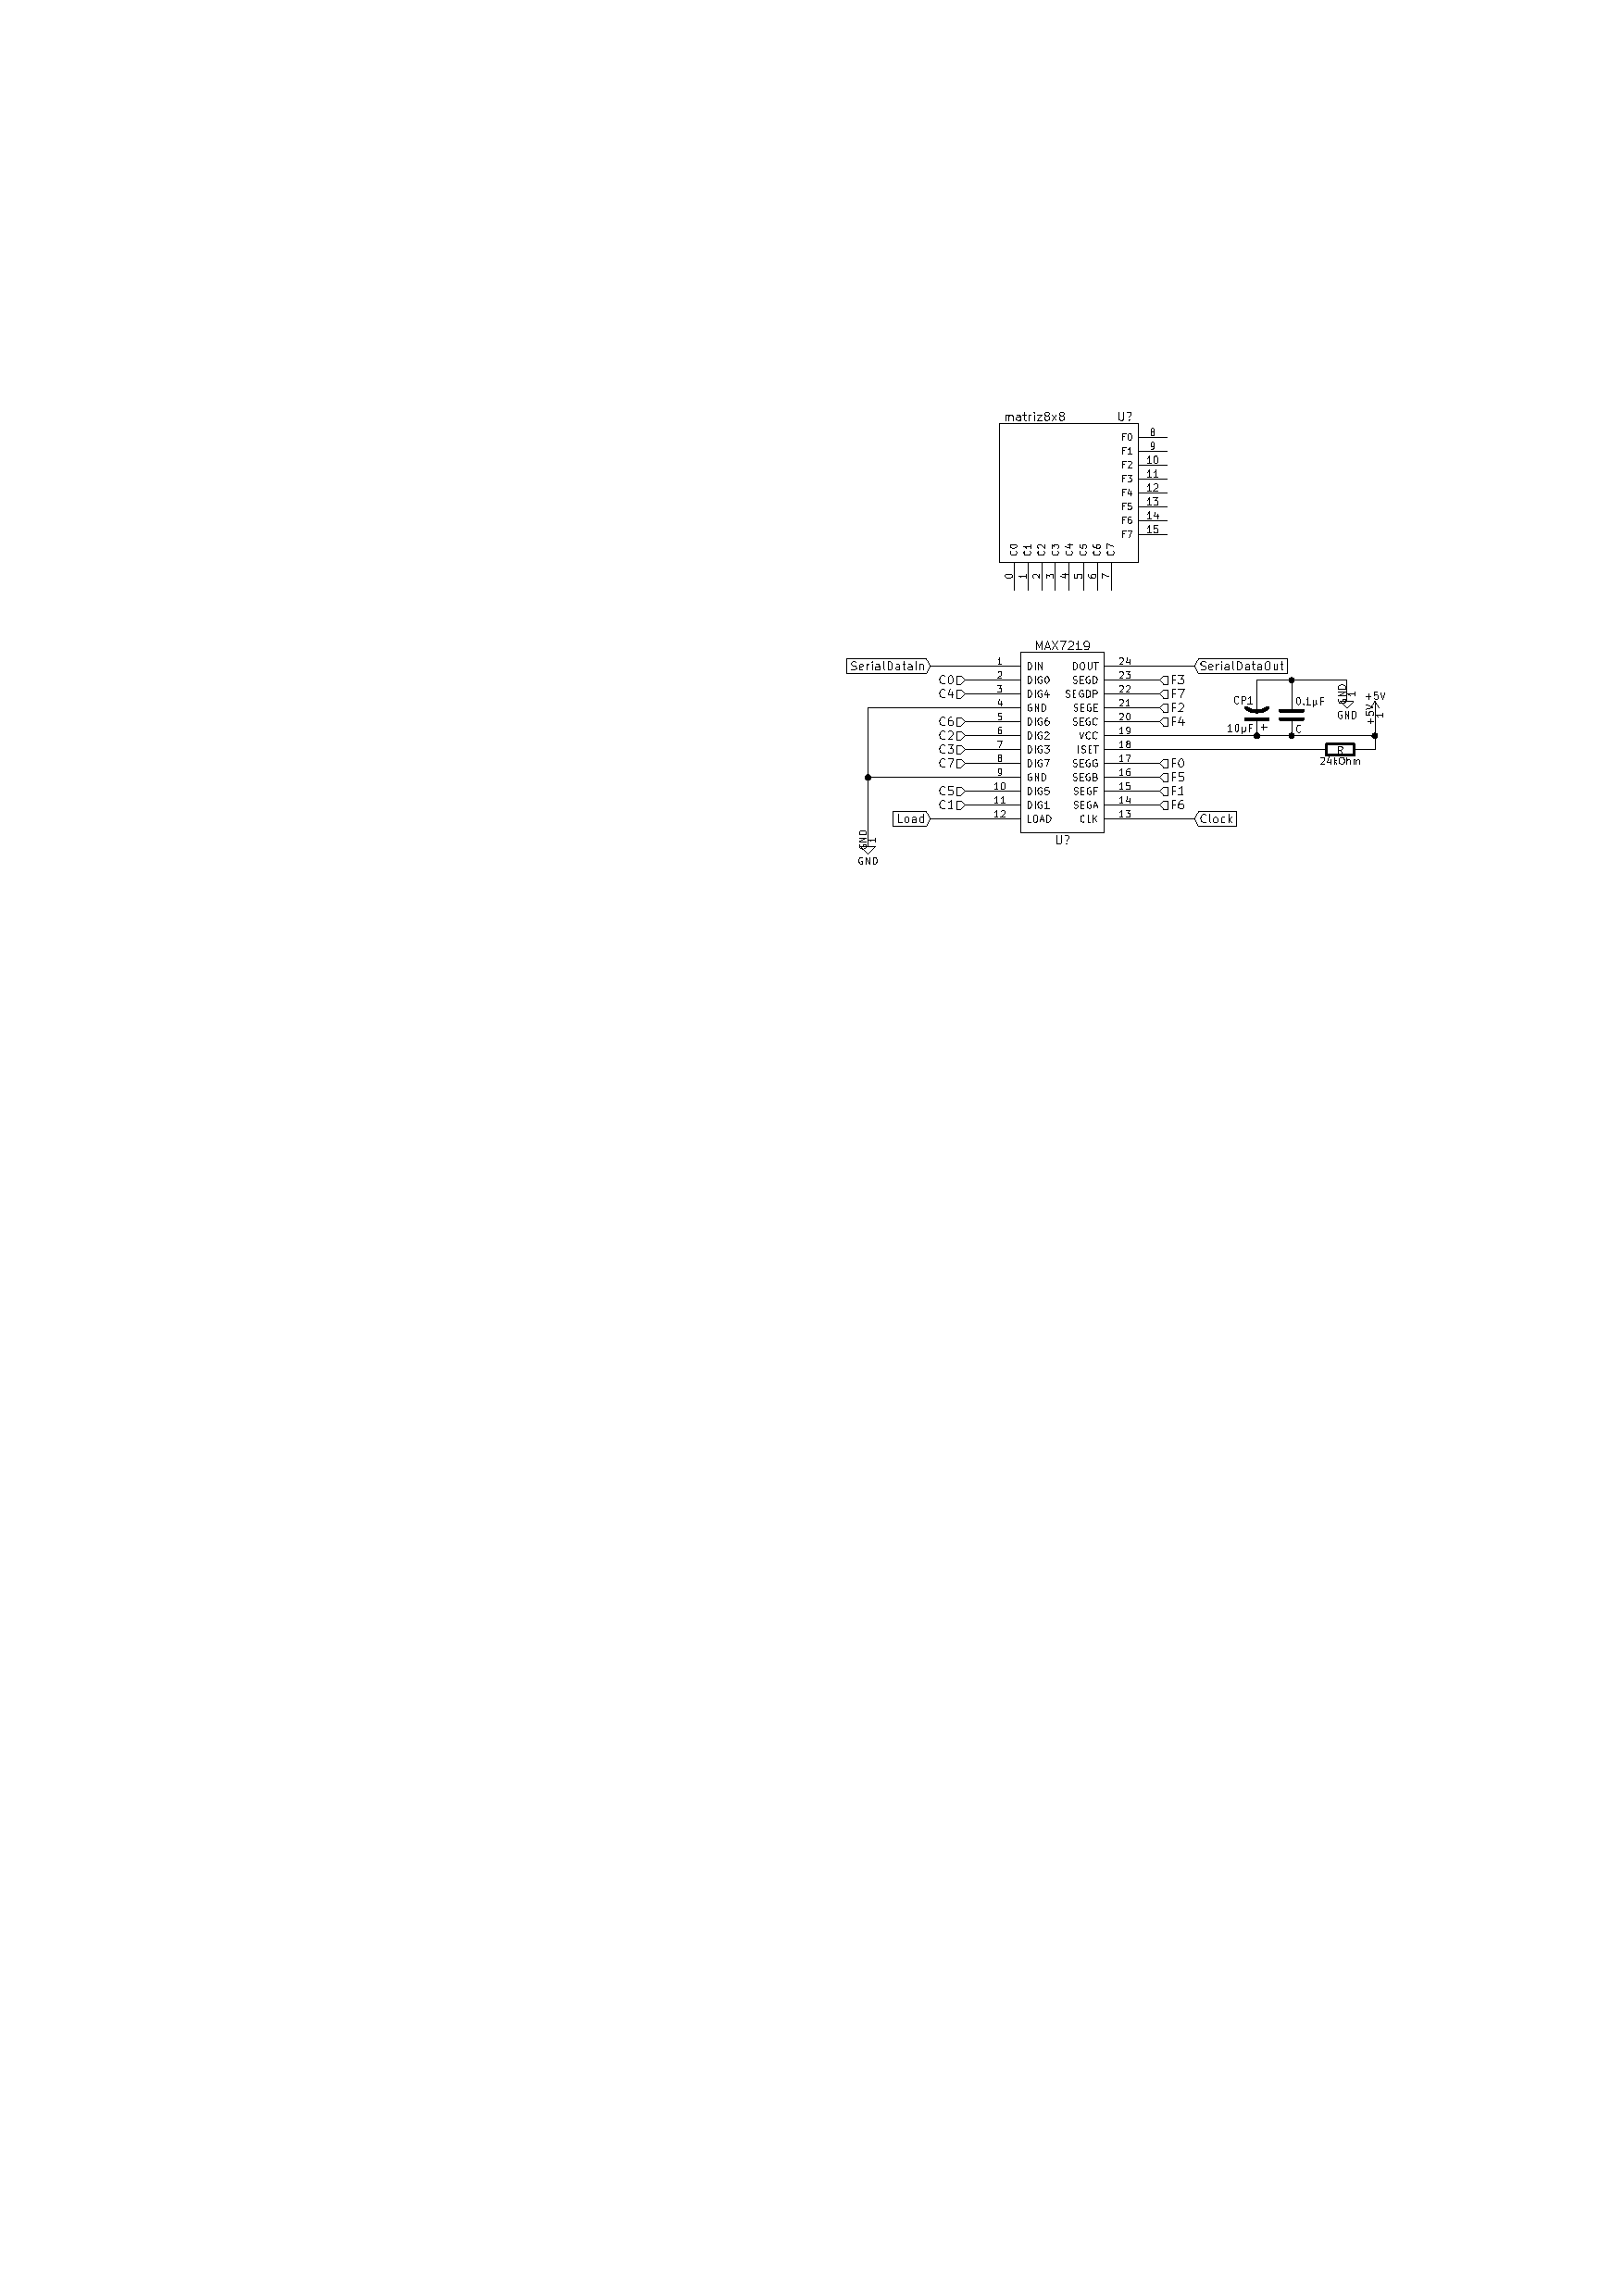
\includegraphics[width=0.8\textwidth]{imagenes/hw/conexion-MAX-matriz.pdf}
	\caption{Conexión entre MAX7219 y su módulo de LEDs.}
	\label{fig:MAX-matriz}
\end{center}
\end{figure}

\begin{figure}[htp!]
\centering
\begin{center}
	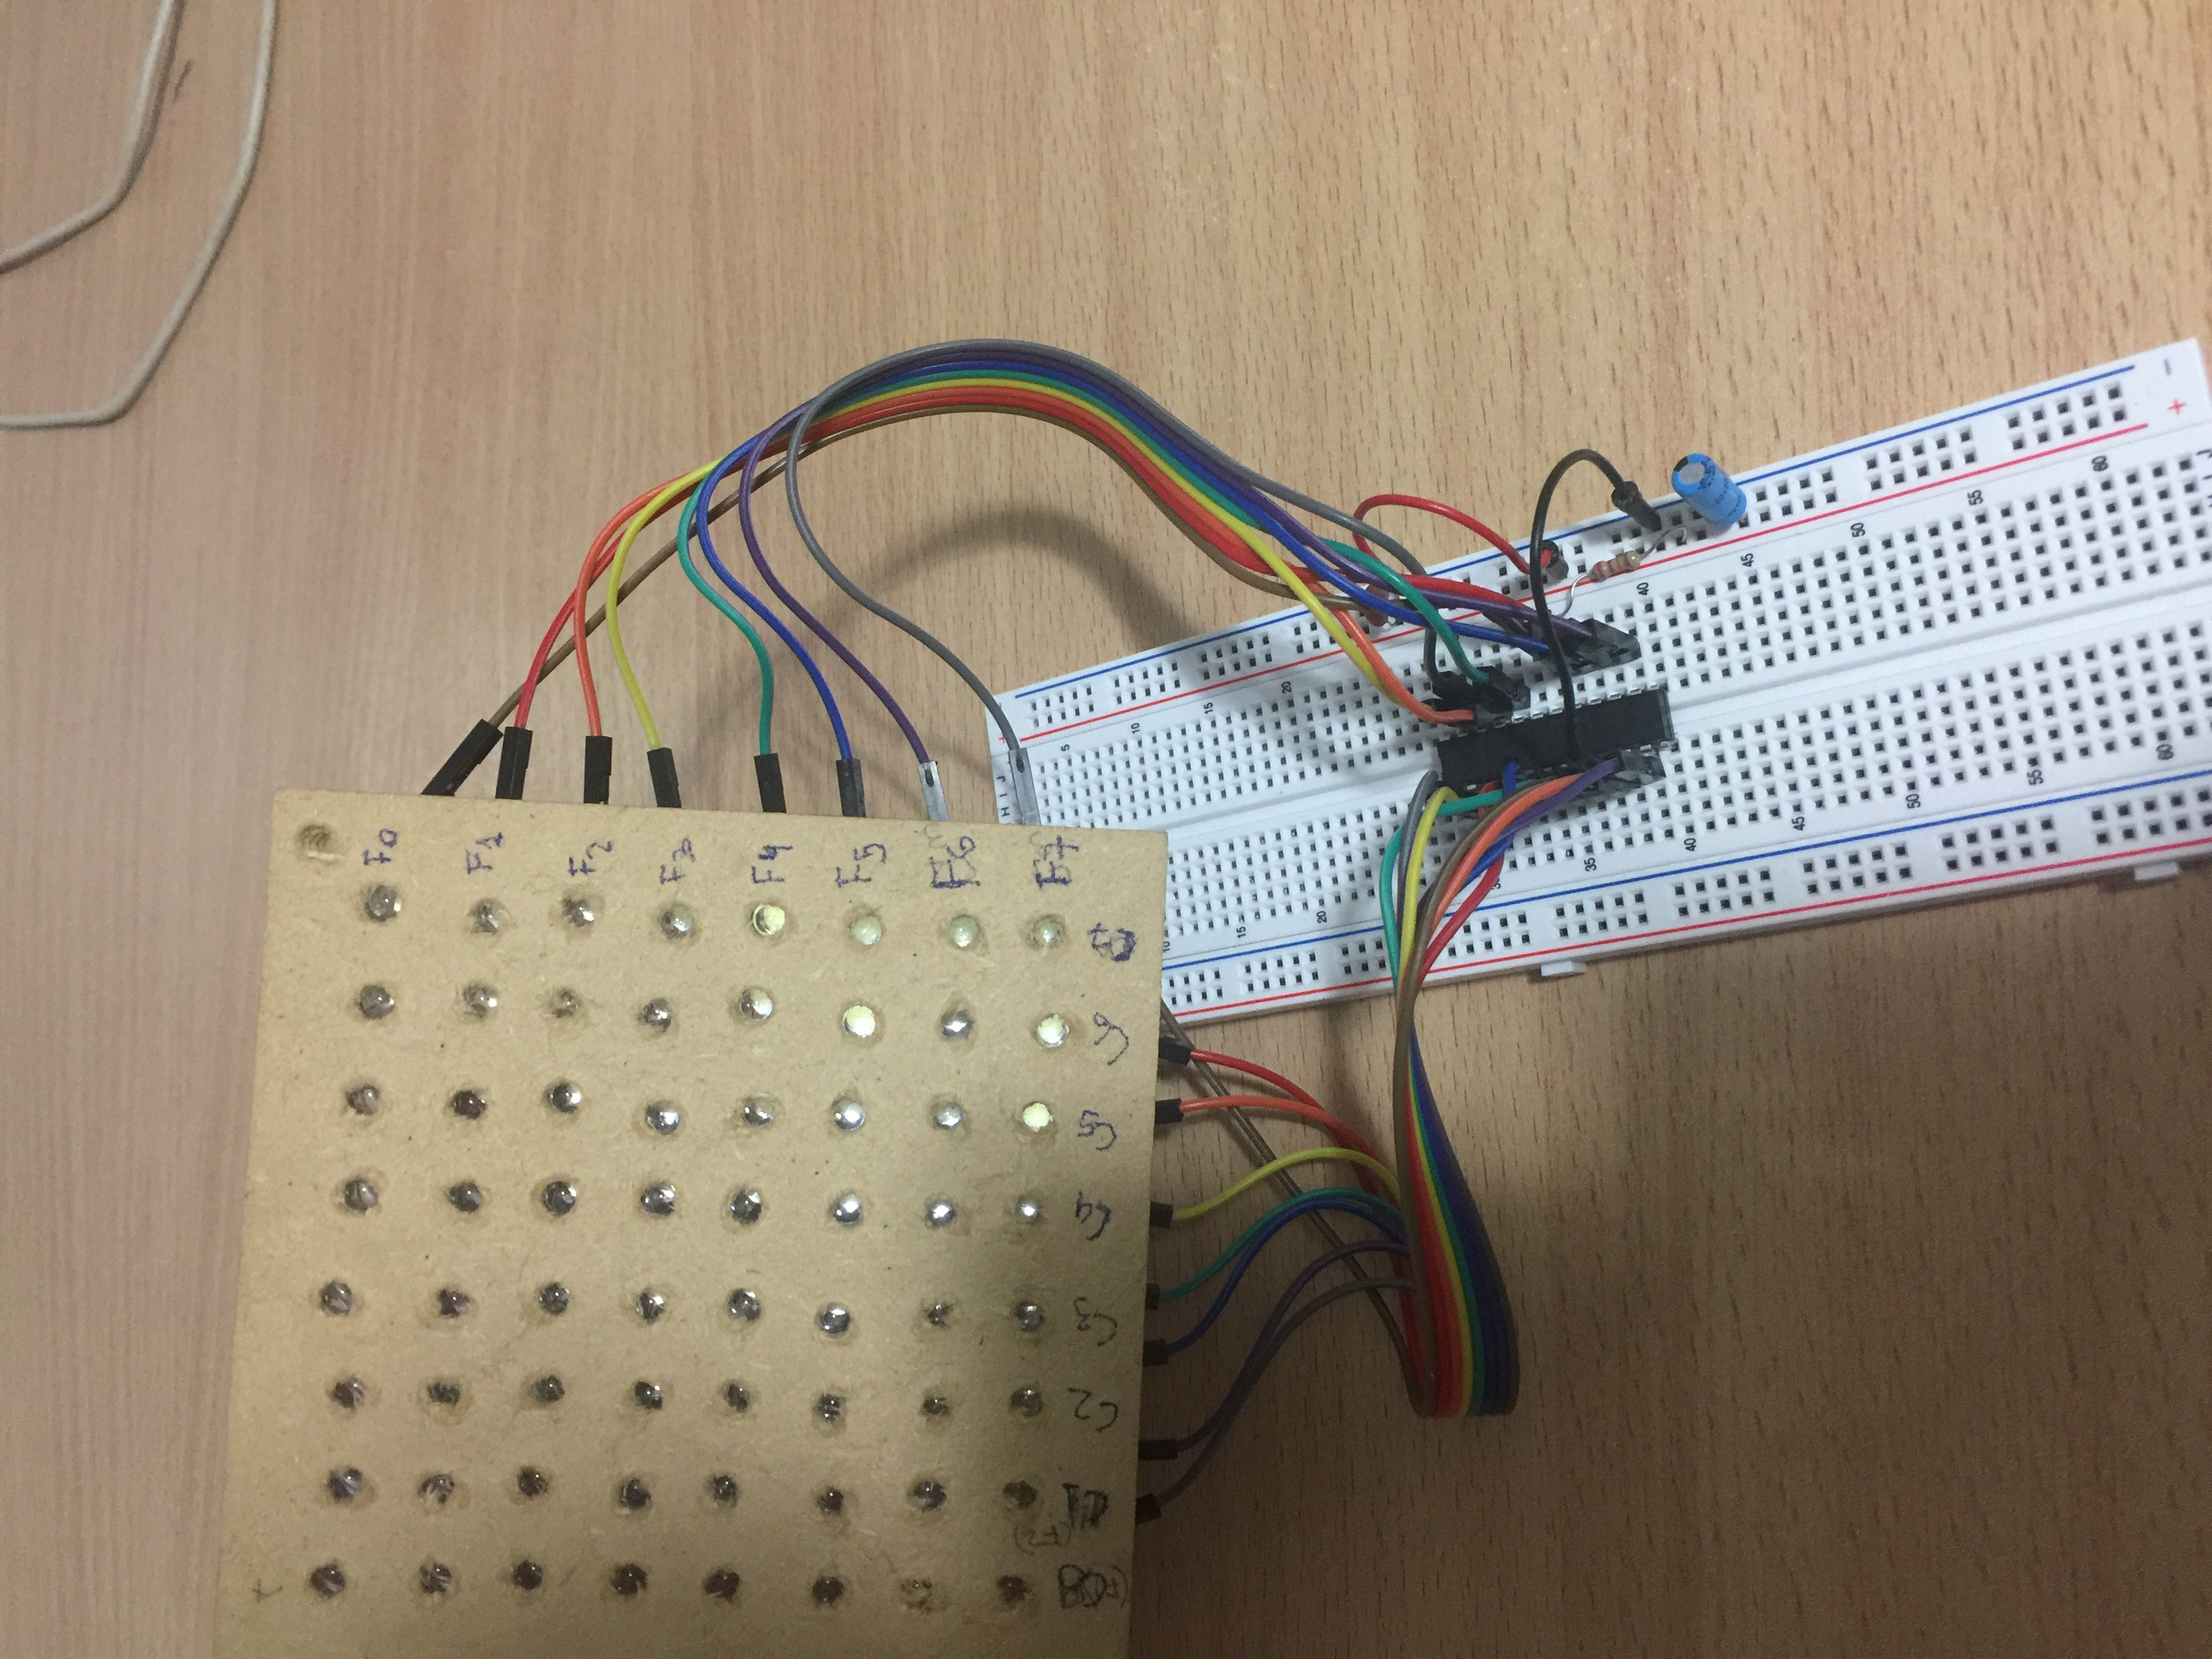
\includegraphics[width=0.7\textwidth]{imagenes/hw/conexion-MAX-matriz.JPG}
	\caption{Fotografía de conexión entre MAX7219 y su módulo de LEDs.}
	\label{fig:MAX-matriz-real}
\end{center}
\end{figure}


\subsection{Matriz de LEDs}
La matriz posee 64 LEDs organizados en ocho filas y ocho columnas, con cátodo común en las columnas como se observa en la figura \ref{fig:modulo-led}. Se analizaron las dimensiones más apropiadas para la utilidad del cartel y se llegó a una separación de 12mm entre LEDs la cual mantiene un dpi apropiado (consiguiendo verse las letras a 10 metros), las demás medidas de pueden observar en la figura \ref{fig:modulo-led-dimensiones}.

Cada uno de los MAX7219 está conectado a una matriz, sus conexiones se pueden observar en el diagrama \ref{fig:MAX-matriz}. Adicionalmente, en la figura \ref{fig:MAX-matriz-real} se observa el prototipo que complementa el esquema de conexión de la figura previamente mencionada.

A la hora de efectuar las conexiones, se debe prestar principal atención a la orientación de la matriz. En la figura \ref{fig:MAX-matriz-real} se indica claramente cuáles son las filas (y su orden) y cuáles son las columnas. Con dicha información el proceso de conexionado se simplifica.

\begin{figure}[!htp]
	\centering
	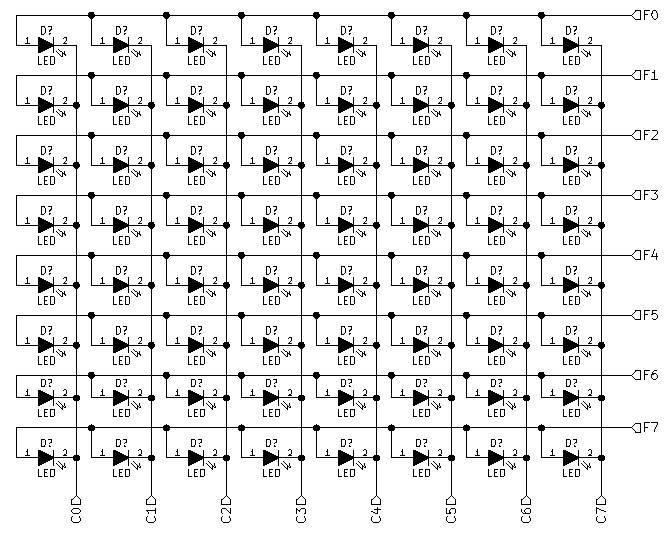
\includegraphics[width=0.7\linewidth]{imagenes/hw/modulo-led.pdf}
	\caption{Esquema de conexiones de la matriz de LEDs.}
	\label{fig:modulo-led}
\end{figure}
\begin{figure}[!htp]
	\centering
	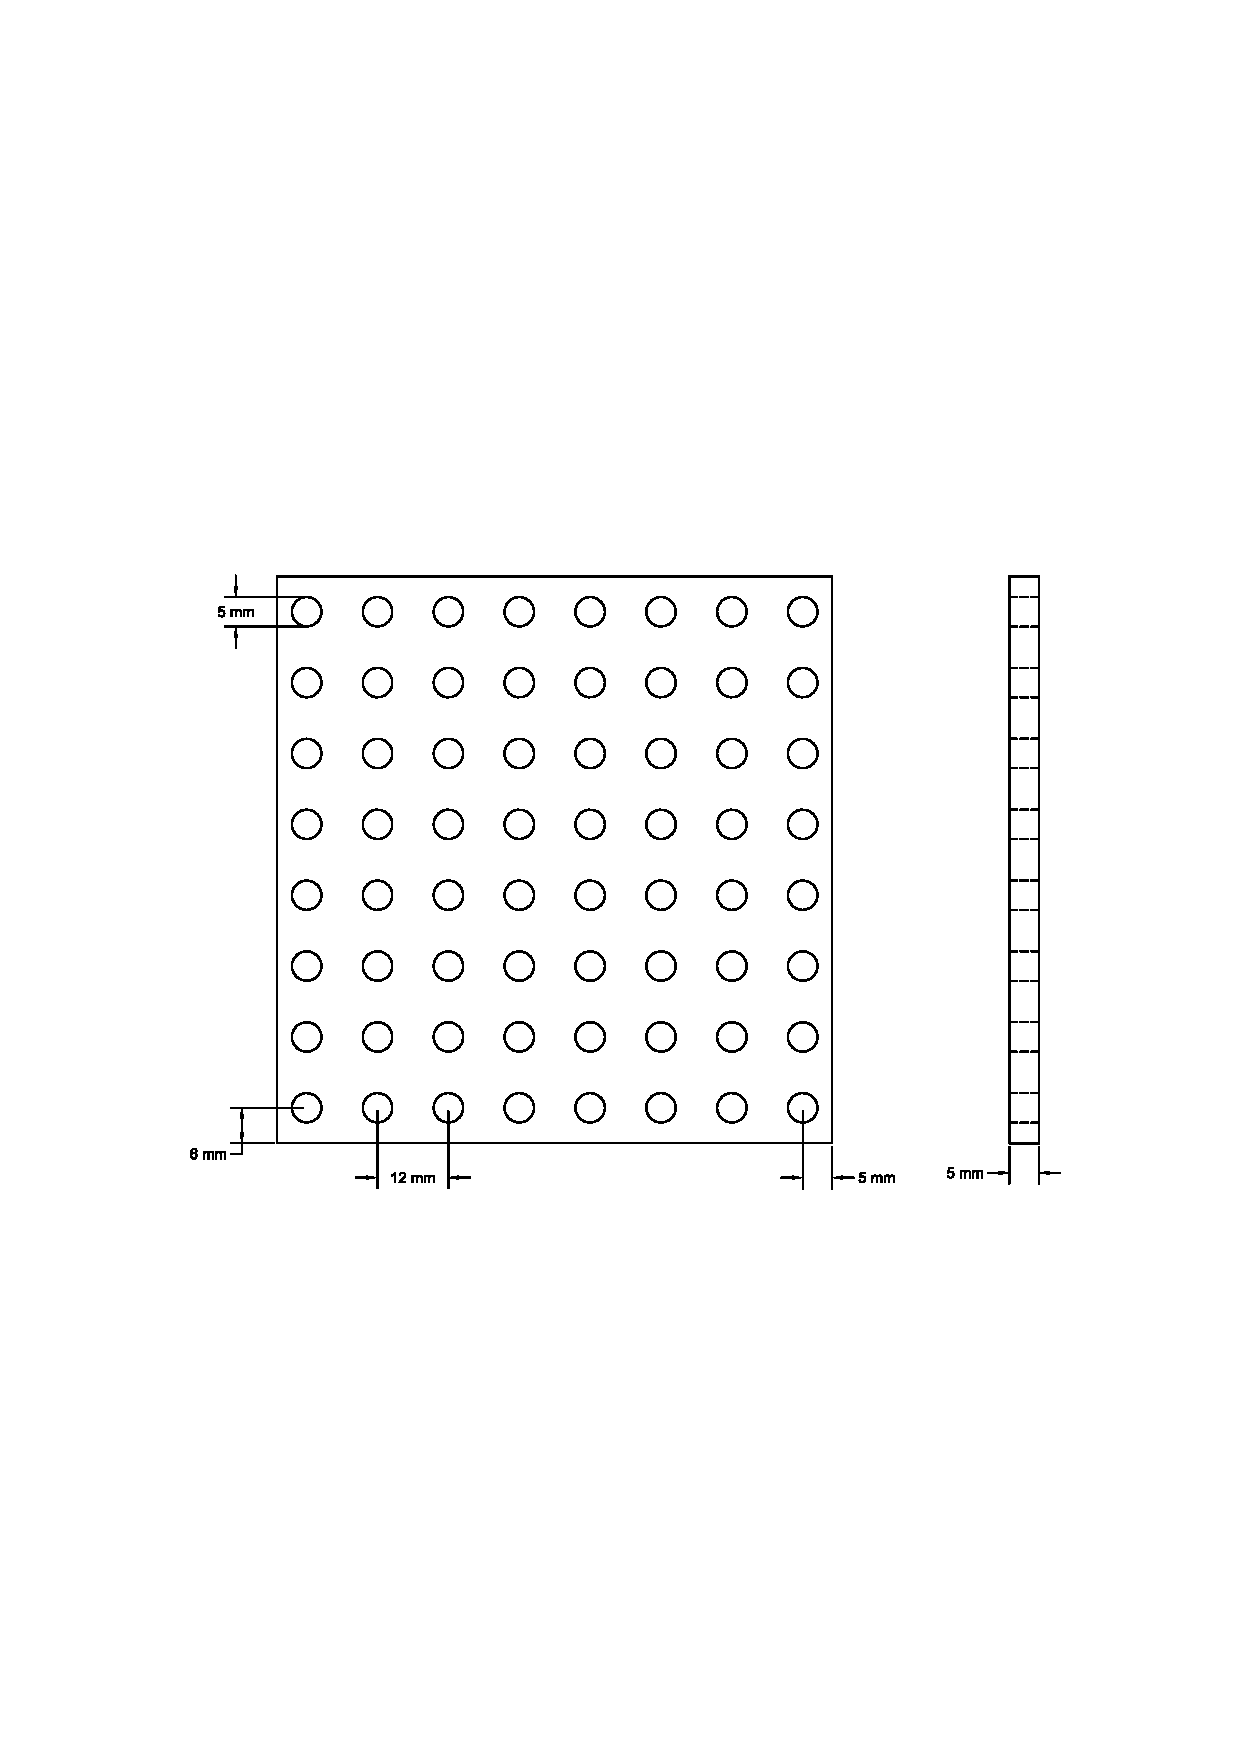
\includegraphics[width=\linewidth]{imagenes/hw/modulo-led-dimensiones.pdf}
	\caption{Dimensiones de la matriz de LEDs.}
	\label{fig:modulo-led-dimensiones}
\end{figure}


\subsection{Comunicación entre los módulos}

\subsubsection{Entre maestro y esclavo}
Como el microcontrolador transmite los datos con un valor alto de 3.3V es necesario convertir estas señales a una tensión que el MAX7219 acepte, la solución que se optó fue incorporar transistores que capaces de transformar 3.3V a 5V. Para ello se conecta tres transistores NPN al circuito, uno por cada señal (DATAIN, LOAD, CLK), se puede observar en la figura \ref{fig:transistors} la conexión de cada transistor con sus respectivas resistencias.

Los transistores utilizados en el prototipo final son los 2N2369. %(http://www.pci-card.com/2n2369.pdf)
La base es el pin 2, el colector el pin 1 y el emisor el pin 3 (ver figura \ref{fig:transistors}).

\begin{figure}[ht!]
	\centering
	\begin{center}
		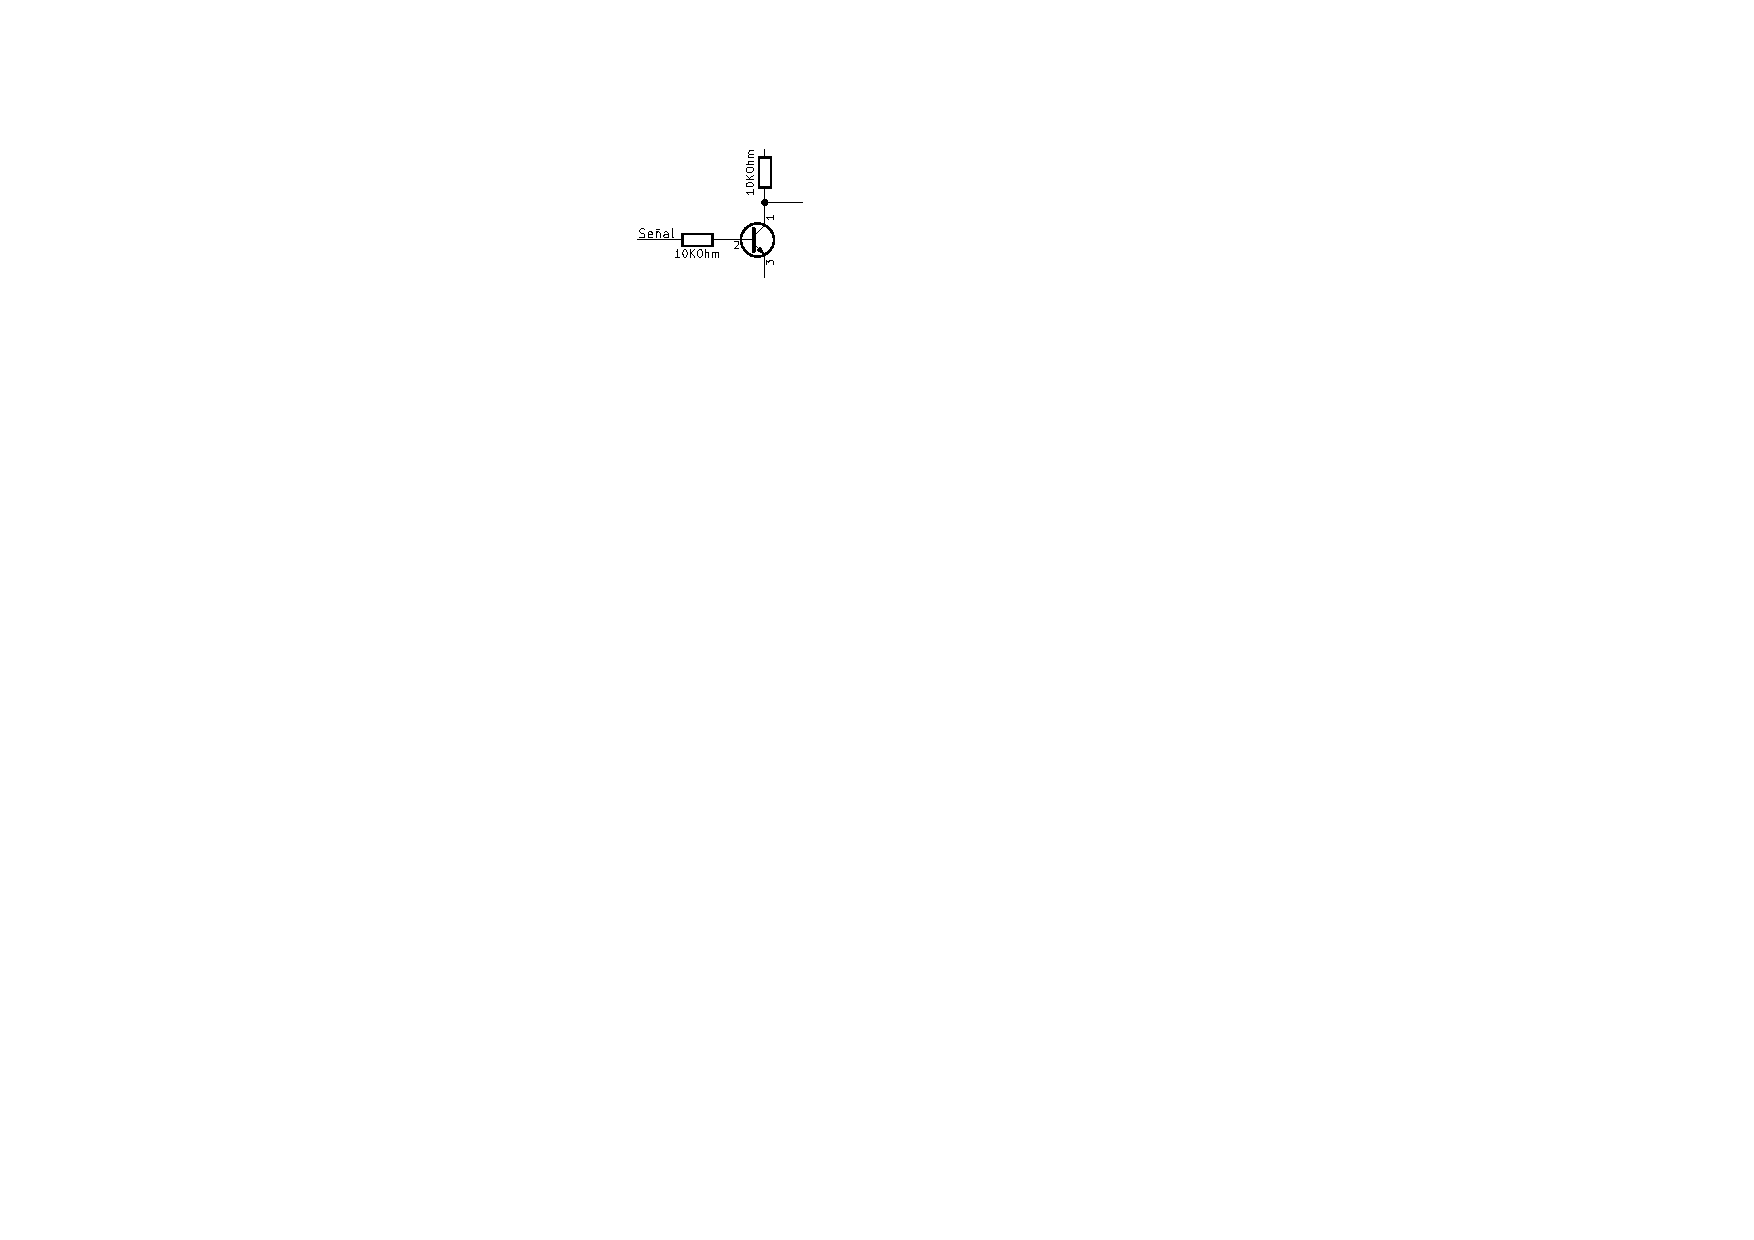
\includegraphics[scale=2]{imagenes/hw/transistor.pdf}
		\caption{Conexión de un transistor, junto con los valores de las resistencias.}
		\label{fig:transistors}
	\end{center}
\end{figure}

\subsubsection{Protocolo de comunicación SPI entre los MAX7219} \label{sec:comunicacion}
Es posible expandir el cartel con N esclavos. En la figura \ref{fig:MAX-MAX} se observa la forma en que se debe realizar la interconexión de los dispositivos integrados.

\begin{figure}[ht!]
	\centering
	\begin{center}
		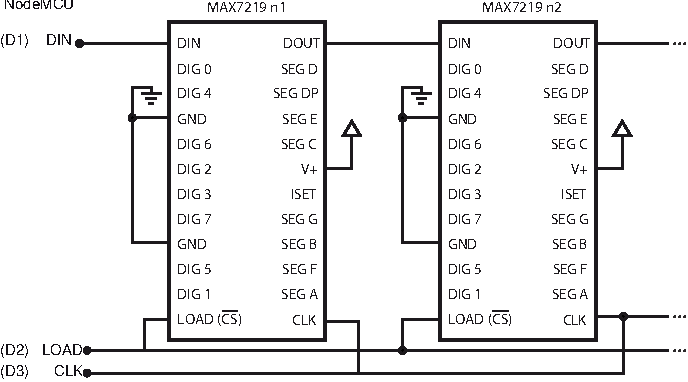
\includegraphics[width=\textwidth]{imagenes/hw/MAX-daisychain.pdf}
		\caption{Conexión entre dos MAX7219.}
		\label{fig:MAX-MAX}
	\end{center}
\end{figure}
Es importante destacar la forma en la que se comunican el microcontrolador con el primer chip shifter, y a su vez, el protocolo que utilizan para comunicarse entre los distintos MAX7219.

La idea general consiste en indicarle a cada chip shifter los leds que debe encender y apagar en cada columna. Para ello debe enviar palabras de dos bytes de manera serial. Es decir, primero envía la información de la columna 1, después la 2, y así siguiendo hasta la 8. El protocolo utilizado es SPI y corresponde a la trama previamente detallada (ver figura \ref{table:trama-spi}).

\begin{table}[ht]
	\centering
	\caption{Trama SPI y su significado.}
	\label{table:trama-spi}
	\begin{adjustbox}{max width=\textwidth}
	\begin{tabular}{|c|c|c|c|c|c|c|c|c|c|c|c|c|c|c|c|}
	\hline
	D15 & D14 & D13 & D12 & D11   & D10   & D9   & D8   & D7 & D6 & D5 & D4 & D3 & D2 & D1 & D0 \\ \hline
	X   & X   & X   & X   & \multicolumn{4}{c|}{ADDRESS} & \multicolumn{1}{c}{ MSB } & \multicolumn{6}{c}{ DATA } & \multicolumn{1}{c|}{ LSB } \\ \hline
	\end{tabular}
	\end{adjustbox}
\end{table}

Para realizar este proceso, la figura \ref{fig:spi-timing-diagram} muestra un diagrama a lo largo del tiempo de la forma de enviar cada bit. En ella se puede observar que el primer paso consiste en bajar la señal de LOAD y esperar un instánte de tiempo (aproximadamente un microsegundo). Luego se debe generar una señal de CLCK de onda cuadrada y de frecuencia de 1Mhz con la mitad de ciclo de trabajo.

El pin conectado al DATAIN del micro, se utiliza para enviar los datos, empezando por el bit más significativo primero. Los datos van a ser leídos por los MAX7219 en el flanco ascendente del CLOCK. Cuando finaliza el envío de los 16 bits, se debe subir la señal de LOAD. En ese momento, el MAX2719 almacena, en sus registros internos, el comando recibido. Todos los comandos son de dos bytes, sin embargo, se puede enviar más de esa cantidad. Esta funcionalidad se utiliza para enviar instrucciones a los demás MAX7219 que están conectados en serie. Lo que ocurre es que la información se recibe en el flanco ascendente de CLK y se envía, hacia el siguiente chip, por el pin DATAOUT en el flanco descendente. De esta forma, en una iteración se pueden configurar una columna de cada módulo de 8x8 LEDs.

\begin{figure}[ht!]
	\centering
	\begin{center}
		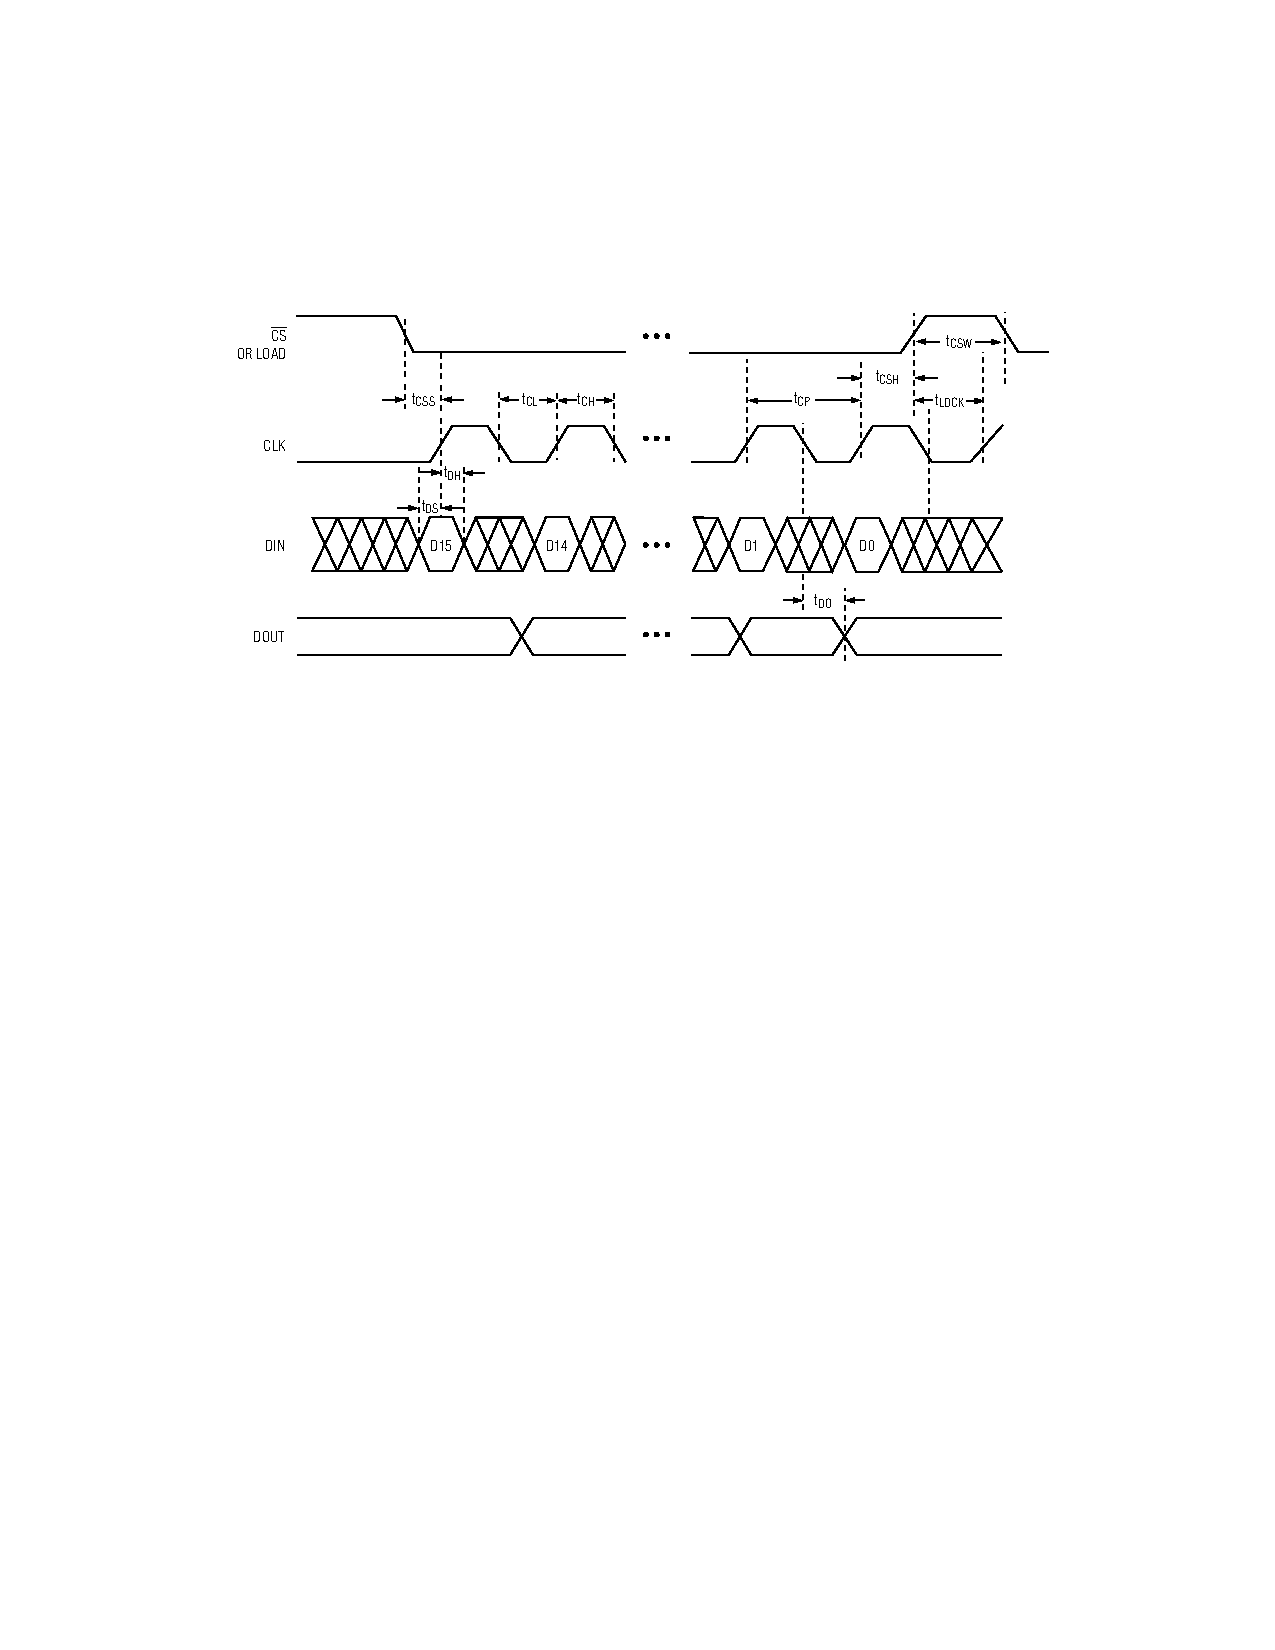
\includegraphics[width=\textwidth]{imagenes/hw/timingDiagram.pdf}
		\caption{Diagrama de tiempo de las señales del MAX7219.}
		\label{fig:spi-timing-diagram}
	\end{center}
\end{figure}



% ========================  Fabricación  ========================



\subsection{Fabricación del circuito PCB}
En ésta sección se menciona como se procedió a la fabricación de los módulos de PCB mediante uno de los métodos mas económicos disponibles, la técnica de transferencia con planchado. Se utilizaron PCB doble cara, destinando una de sus caras para una superficie GND que unifique la conexión de todos los nodos de tierra de la placa.

Este proceso consiste en cinco pasos esenciales, que serán detallados a continuación con detalles sobre como se debería proceder, las buenas practicas y sugerencias en cada paso.

\subsubsection{Pasos preliminares}
Antes de empezar es necesario contar con todos los materiales a utilizar. En el apéndice \ref{sec:materiales} se indica la lista de todos los componentes y materiales que se requieren en los procesos.

En primer lugar, con el papel ilustración se imprime el dibujo del circuito (un ejemplo de éste, se encuentra en la figura \ref{fig:imp-pcb} del apéndice \ref{sec:materiales}), con una impresora laser. Se recomienda dejar un borde excedente para facilitar el proceso de planchado. Prestar mucha atención, que al imprimir el circuito mediante este método, la imagen del mismo se espeja al planchar.

Antes de pasar al siguiente paso, es necesario quitar toda grasitud y suciedad de la plancha de cobre, con detergente (no con alcohol) y virulana fina, para evitar que impidan la correcta adhesión de la tinta durante el planchado.

\subsubsection{Planchado}
Apoye la plancha de cobre sobre una superficie firme no inflamable. Retire de la cercanía todo objeto que pueda obstruir sus movimientos durante el planchado. Posicione el papel lo más centrado posible boca abajo en la plancha de cobre. Asegurese de que el papel está apoyando bien sobre toda la plancha, y proceda a presionar con la plancha unos pocos minutos en la zona del dibujo previamente impreso. El papel no debe tener síntomas de quemaduras, si esto ocurre inmediatamente quitar la plancha ya que podría arruinar toda la transferencia de la tinta.

Tras haber realizado esto durante unos 10 a 15 minutos (el tiempo puede variar según el calor de la plancha y la calidad del papel), retire la misma, desconecte su cable de alimentación y luego sumerja en un recipiente con agua fría la placa con la hoja que en este punto estará adherida a la misma. Deje reposar unos minutos hasta que se enfrien. Pasados unos 5 minutos, el calor ya se habrá disipado lo suficiente como para proseguir. Retire la placa y el papel del agua, apoyelos sobre un trapo seco sobre una superficie firme, y con las yemas de los dedos retirar el papel con mucho cuidado de no producir rayaduras y evitando que se salga la tinta, que ahora estará pegada al cobre.
En la figura \ref{fig:sacado-papel} se observa como se va quitando el papel.

\begin{figure}[ht!]
	\centering
	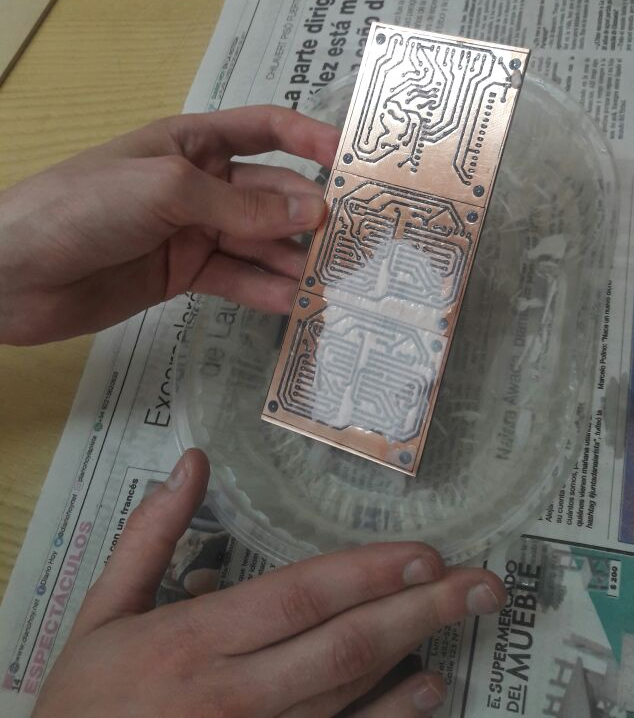
\includegraphics[width=0.6\linewidth]{imagenes/pcbeando/sacado-papel-1.png}
	\caption{Proceso de quitar el papel.}
	\label{fig:sacado-papel}
\end{figure}

\subsubsection{Reducción del Cobre}
Una vez quitado todo el papel fotográfico debería quedar solo la tinta impregnada en el cobre (ver figura \ref{fig:pos-sacado-papel-1}). Si de alguna manera se salió la tinta, es posible corregir las imperfecciones con un marcador de esmalte, en la parte superior izquierda de la figura se puede notar que se requirio corregir el agujero del tornillo.

\begin{figure}[ht!]
	\centering
	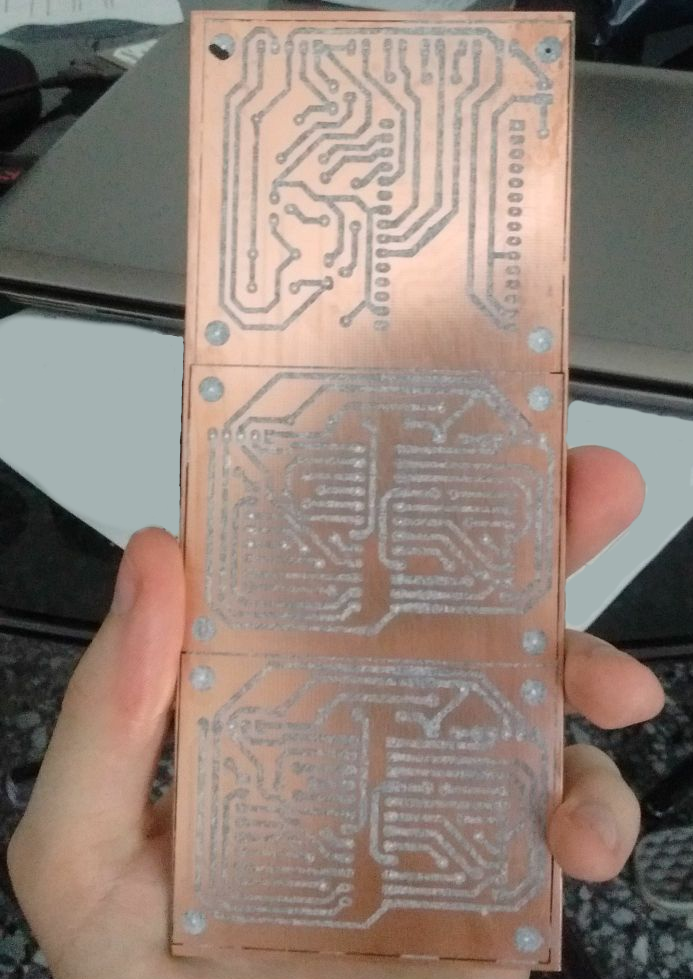
\includegraphics[width=0.47\linewidth]{imagenes/pcbeando/pos-sacado-pape-1.png}
	\caption{Pos sadcado papel.}
	\label{fig:pos-sacado-papel-1}
\end{figure}

{ \color{red} Contar que se opto por hacer GND toda una cara por lo tanto habia que pintar con esmalte la otra cara para que el cobre no lo comiera }

En la figura \ref{fig:pos-sacado-papel-2} se puede ver el resultado luego de aplicar esmalte.

\begin{figure}[ht!]
	\centering
	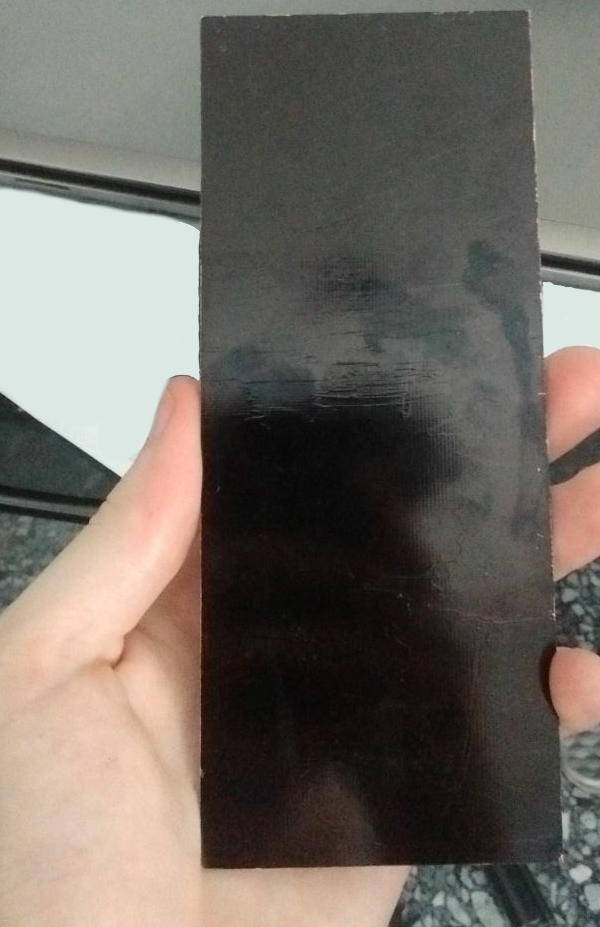
\includegraphics[width=0.47\linewidth]{imagenes/pcbeando/pos-sacado-papel-2.png}
	\caption{Pos sadcado papel 2.}
	\label{fig:pos-sacado-papel-2}
\end{figure}

Para reducir el cobre utilizar guantes de latex ya que el acido ferrico mancha. 


{ \color{red} Contar el procedimiento del acido, de que no hay que mover mucho y dejar reposar al menos 15 min si el acido esta usado. En un ambiente abierto (y sobre todo sin vientoo (?..), sobre una superficie en la que si se derrama no pasa nada... cuando ya esta comido lavar con abundante agua para quietar el acido y dejar secar por al menos 10 minutos.
Contar tambien que se utilizo un hilo enganchado para evitar tocar la placa directamente. }
En la figura \ref{fig:acido} se muestra la placa cubierta de acido sostenido por un hilo azul que se utilizo como ayuda para sacarlo del recipiente.
\begin{figure}[ht!]
	\centering
	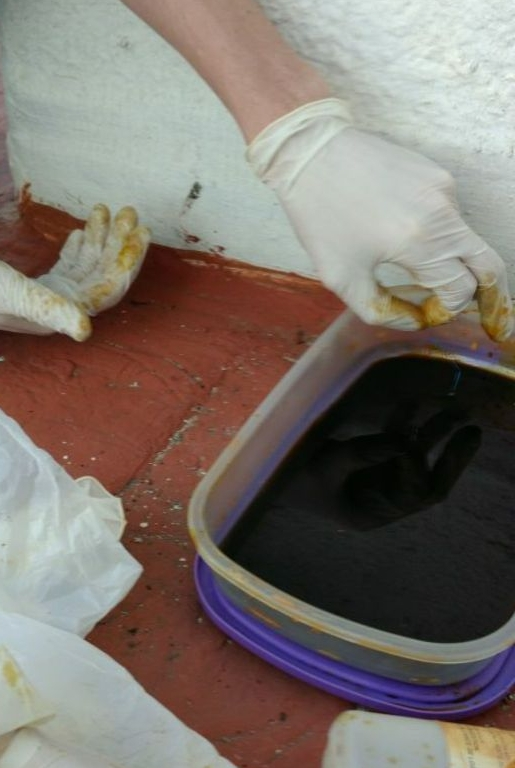
\includegraphics[width=0.4\linewidth]{imagenes/pcbeando/acido.jpeg}
	\caption{Acido}
	\label{fig:acido}
\end{figure}


En la figura \ref{fig:pos-acido} se observa el resultado de ese paso.

\begin{figure}[ht!]
	\centering
	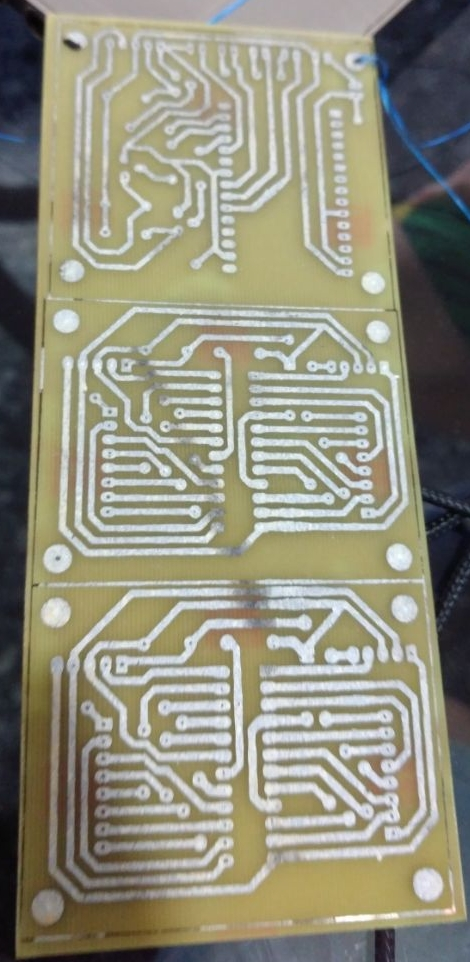
\includegraphics[width=0.36\linewidth]{imagenes/pcbeando/pos-acido-2.jpeg}
	\caption{Pos acido}
	\label{fig:pos-acido}
\end{figure}

\subsubsection{Perforado de Placas}
En este paso se requieren las mechas especificadas en el apéndice \ref{sec:materiales-para-hacer-cartel}. Es importante contar con mechas de las medidas ya que cada componente posee diferente tamaño de pines. La correcta elección de diámetro para cada uno contribuye a que el proceso de soldado sea menos trabajoso y disminuye la posibilidad de que la soltura de un componente entorpezca dicho paso provocando un mal funcionamiento del sistema.

Antes de proseguir con el siguiente paso se realizaron los cortes pertinentes de forma de separar los módulos entre sí. Utilizando una sierra de arco, en primer lugar se marcó la línea de corte para facilitar el proceso.
Luego con mucho cuidado se procedió con la misma. Seguido de esto, es recomendable que se lijen los bordes de los PCB para evitar futuros accidentes ya al cortarlo con una sierra queden imperfecciones filosas.

En la figura \ref{fig:pos-corte} se muestran como deberían quedar los módulos lijados y separados entre sí.

\begin{figure}[ht!]
	\centering
	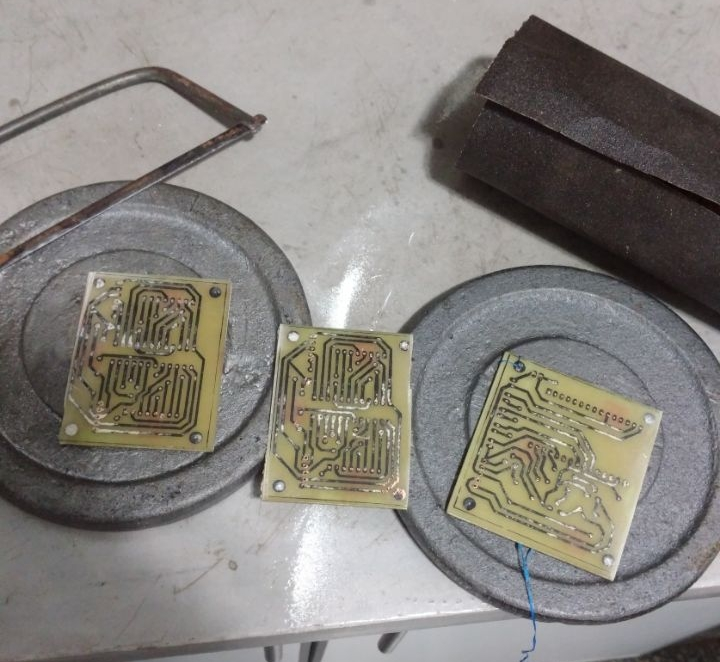
\includegraphics[width=0.7\linewidth]{imagenes/pcbeando/pos-corte.jpeg}
	\caption{Pos corte}
	\label{fig:pos-corte}
\end{figure}

\subsubsection{Montaje}

{ \color{red} Finalizando la fabricación, en primer lugar se monta los pines que seran el soporte a los componentes, por ejemplo el NodeMCU del master será conectado a dos tiras de pines de NxN pines para que el mantenimiento del modulo sea mas flexible.
Se recomienda probar las conexiones de los componenetes antes de seguir con el montaje del siguiente para evitar fallos indeseados (en soft seria test unitario).}


%TODO esto no tiene formato de lista ni espaciado, halp pls%

\subsection{Manual de instalacion de hardware}

%TODO deberia esto ir aca al final o seccion nueva? La fabricacion tambien on deberia ser seccion nueva?%

Para compenzar con la instalacion del hardware, identifique cada uno de los modulos a instalar. El módulo maestro puede diferenciarse facilmente porque no posee una pantalla, además de que cuenta con una ficha de alimentación que los módulos esclavo no poseen. Los módulos esclavo en cambio cuentan con una matriz de LEDs.

%Dibujo basico de modulos %


Determine donde va a instalar el cartel. La altura ideal para su instalación es montado sobre la pared a una altura de alrededor de 1.80 metros. Esta altura garantiza su facil divisación por parte de personas de todas las estaturas sin resultar molesto de ver para ninguna en particular. El cartel deberá montarse sobre una pared preferiblemente despejada, en un area donde haya un tomacorrientes de 220 V a una distancia no mayor a 1 metro -debido al largo del cable de alimentación de la fuente incluída-, y lejos de cualquier fuente de luz directa cuyo reflejo pueda afectar la legibilidad del mensaje mostrado por el cartel. Esto también implica que para su óptima legibilidad, el cartel debe ser instalado en espacios interiores, siendo su potencia lumínica insuficiente para garantizar la correcta legibilidad de los mensajes bajo la luz solar directa.

%Dibujo basico de pared con tomacorrientes cerca, linea punteada con cartel a la altura adecuada. Puede ser complicado, en cuyo caso mejor no lo hacemos %


Apoye sobre una mesa los modulos, uno al lado de otro, simulando el orden en el que quedarán sobre la pared. Esto le permitirá identificar el ancho del cartel para saber si puede montarlo correctamente en el espacio disponible. Luego apoyando de a dos modulos sobre la pared, marque las posiciones donde el gabinete permite que pasen los tornillos para sujetarlos. Repita para todo para subsecuente de módulos hasta haber hecho las marcas para todos.


%Dibujo basico de modulos sobre pared e indicacion sobre donde irian los tornillos %


Una vez hechas las marcas haga los agujeros para poner los tarugos donde quedaran sujetos los tornillos. No utilice tornillos más finos de los indicados ya que estos pueden no soportar el peso del cartel.


Apoye los modulos en la pared de manera que coincidan los agujeros de guia con los agujeros realizados, y luego inserte los tornillos en los mismos y ajustelos. El cartel tendria que quedar fijo y estatico en el lugar tras haber realizado esto.


Conecte con los cables provistos el módulo maestro con la interfaz de entrada del primer modulo esclavo. Luego la interfaz de salida del primer modulo esclavo con la interfaz de entrada del segundo modulo esclavo. En caso de haber más módulos esclavo, repita este último paso hasta que todos estén conectados en cadena.

Conecte la fuente de alimentacion en un tomacorrientes de 220V y en la ficha de alimentación del módulo maestro.

El cartel ya se encuentra instalado y listo para su configuración y uso.
